\documentclass[10pt,letterpaper]{article}
\usepackage{ifpdf}
\usepackage{graphicx}
\usepackage{xcolor}
\usepackage{microtype}
\usepackage[T1]{fontenc}
\usepackage[sfdefault]{overlock}
\usepackage{cancel}
\usepackage{url}

\ifpdf
  \pdfpagewidth=\paperwidth
  \pdfpageheight=\paperheight
\fi

\setlength\oddsidemargin{-0.1in}
\setlength\evensidemargin{\oddsidemargin}
\setlength\textwidth{\paperwidth}
\advance\textwidth-2in
\advance\textwidth-2\oddsidemargin
\setlength\topmargin{-0.5in}
\setlength\topskip{0in}
\setlength\headheight{0in}
\setlength\headsep{0in}
\setlength\textheight{9.5in}

\pagestyle{empty}

\begin{document}
\begin{center}
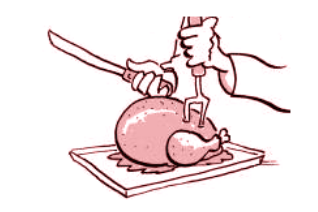
\includegraphics[width=1.5in]{../../../images/logo.png} \\
{\large\bfseries The 5th Annual Workshop on} \\[5pt]
{\LARGE\bfseries Forming an Ecosystem Around Software Transformation (FEAST)}\par
\end{center}

The
2020
Workshop on Forming an Ecosystem Around Software Transformation (FEAST) will be held in conjunction with the ACM Conference on Computer and Communications Security (CCS) on
November 13th, 2020.
The workshop is geared toward discussion and understanding of several critical topics surrounding software executable transformation for improving security and efficiency of all software used in security-critical applications.
The scope of discussion will include topics that may be necessary to fully exploit the power and impact of late-stage software customization.

\section*{Call for Papers}

The 5th Workshop on FEAST
seeks submissions presenting novel contributions, works in progress, position papers, challenge papers, and systematization of knowledge papers
concerning all aspects of late-stage customization and analysis of binary executable software for security.
Authors are encouraged to submit papers that will foster discussion and highlight emerging challenges and novel approaches to achieving effective, robust transformation and analysis of binary code with little or no reliance on source code.

Typical software engineering methodologies are largely focused on programmer productivity for delivering general-purpose software to the widest possible set of consumers.
While this approach maximizes profits, it tends to yield
software that is bloated with features that might pose unnecessary risks for security-sensitive consumers,
code that is unnecessarily inefficient in terms of time and space overheads,
and/or software that sacrifices security and reliability assurances.

Recent work has sought to undo these disadvantages by innovating facilities for (semi-)automatically analyzing and customizing the binary code purveyed by software vendors without reliance on developer-owned source code.
Customizations of interest include (but are not limited to)
program specialization (de-bloating),
reduction of levels of indirection (de-layering),
control-flow and dataflow simplification (complexity reduction),
binary optimizations related to the above (streamlining),
and techniques for achieving higher assurance for customized code (e.g., formal methods).
Numerous promising results from these efforts have demonstrated their viability for improving program execution efficiency as well as reduction of the cyber security attack surface.
Further advances in these areas will benefit the community by investing in the development of tool ecosystems to take advantage of this recent progress, to mature the technologies, and to determine how best to transparently deploy them.

Despite this ongoing progress within the research community,
software executable transformation is not a solved science.
Some critical problems of reverse engineering and binary analysis are
provably undecidable in the general case.
Various automated tools and ecosystems still need to be investigated and developed to guarantee the effectiveness and correctness of transformation efforts,
and to enhance and ensure the security of transformed software.
In addition, emerging challenges deserving special attention of the research community must be identified, and the relative merits of existing knowledge must be systematized.
The FEAST workshop will therefore include topics geared toward:
\begin{itemize}
\item understanding issues of software executable transformation for various programming languages and environments, and the potential methods for alleviating those issues;
\item identification of tools to be investigated and developed for guaranteeing correctness, enhancing security, and enabling non-critical, undesired feature removal;
\item identification of layers and areas of computing systems that are suitable for (and can benefit from) software customization and/or transformation,
along with the identification of associated challenges and constraints,
and the particular adaptation to the methodology needed to operate within the identified areas; and
\item automated extraction of models from software executables that are amenable to formal methods analysis and verification.
\end{itemize}

Submissions should be in two-column, 10-point format, double-blind, and can be up to 6 pages in length with as many additional pages as necessary for references.
Authors should submit their papers at
\url{https://feast20.hotcrp.com}.

\section*{Important Dates}

{\large
\begin{itemize}
\item \textbf{July \cancel{17} 24, 2020 AOE:} Submission deadline
\item \textbf{August 12, 2020:} Author notification
\item \textbf{September 2, 2020:} Camera-ready deadline
\item \textbf{November 13, 2020:} Workshop date
\end{itemize}
}

\section*{Program Committee}

\begin{itemize}
\item Long Lu, Northeastern University (co-chair)
\item Kevin Hamlen, The University of Texas at Dallas (co-chair)

\item Michael Brown, Georgia Institute of Technology
\item Lorenzo De Carli, Worcester Polytechnic Institute
\item Michael Franz, University of California at Irvine
\item Vasileios Kemerlis, Brown University
\item Tian Lan, George Washington University
\item Byoungyoung Lee, Seoul National University
\item Zhiqiang Lin, Ohio State University
\item Jiang Ming, The University of Texas at Arlington
\item Michalis Polychronakis, Stony Brook University
\item Eric Schulte, GrammaTech
\item Nik Sultana, University of Pennsylvania
\item Guru Venkataramani, George Washington University
\item Maverick Woo, Carnegie Mellon University
\item Dinghao Wu, The Pennsylvania State University
\item Wenfei Wu, Tsinghua University
\end{itemize}

\end{document}

